% Anexo independiente. Cálculos nominales; no aprobación de fabricación.
\section{Memoria de cálculo del prototipo manual}
\subsection{Presión y preparación de material}
Los argumentos de la exponencial son adimensionales; $P_{N0}$ fija la unidad de presión.
La relación CAD exacta es $10/6$; el valor redondeado $1,667$ da $2,25938\,\mathrm{MPa}$.
El cociente con $43,70\,\mathrm{MPa}$ es aproximadamente $0,0517$.
La diferencia de $0,30\,\mathrm{MPa}$ respecto a los $44\,\mathrm{MPa}$ de EP2 está identificada;
la ecuación4 de EP2 da $43,70433\,\mathrm{MPa}$ al usar $L/D=6$, justificando ambos redondeos.
El canal restrictivo CAD comercial es $31,5\,\mathrm{mm}$, mientras el predimensionamiento usa
$36\,\mathrm{mm}$; no se modifica retrospectivamente la presión44MPa de sus simulaciones.
\begin{equation}m_w=m_0\frac{w_f-w_0}{1-w_f}.\end{equation}
\subsection{Equilibrio y resistencia nominal}
\begin{align}
F_i&=P A_{i,\mathrm{cubierta}},&T&=\sum_i\mu_{\mathrm{ef}}F_i r_i,\\
R_a&=F\frac{x_b-x_F}{x_b-x_a},&R_b&=F-R_a,\\
\mathbf K\mathbf u&=\mathbf f,&I&=\frac{\pi d^4}{64},\\
\sigma_b&=\frac{32M}{\pi d^3},&\tau_{V,\max}&=\frac{16V}{3\pi d^2}.
\end{align}
La flexión máxima superficial y el corte máximo central no están co-localizados;
no se combinan sus envolventes como un estado real de von Mises.
El umbral nominal $S_{y,\mathrm{req}}=\sigma_{b,\max}$ para $n=1$ no incluye entallas ni reserva de diseño.
Los ciclos de fibra fija dan $\sigma_m=(\sigma_{\max}+\sigma_{\min})/2$ y
$\sigma_a=(\sigma_{\max}-\sigma_{\min})/2$. Un criterio posterior de Goodman requeriría
$K_f\sigma_a/S_e+K_t\max(\sigma_m,0)/S_{ut}\leq1/n$, según EP2 ecuación38, y correcciones documentadas;
no se asignan esos valores al material desconocido.
El cribado usa el rango de extremos de una vuelta en 16 direcciones fijas, no un conteo rainflow
ni daño acumulado. EP2 empleó 144 fibras y rainflow; sus resultados resistentes no se transfieren.
\begin{table}[ht]\centering\begin{tabular}{rrrrr}\toprule
Capa [mm]&$d$ [mm]&$\sigma_b$ [MPa]&$u_{\max}$ [mm]&$\Delta g_{\max}$ [mm]\\\midrule
1 & 4.773 & 456.00 & 1.206 & 1.166\\
1 & 6.000 & 229.55 & 0.483 & 0.467\\
2 & 4.773 & 751.15 & 1.980 & 1.915\\
2 & 6.000 & 378.13 & 0.793 & 0.767\\
4 & 4.773 & 1121.97 & 2.952 & 2.854\\
4 & 6.000 & 564.81 & 1.182 & 1.143\\
\bottomrule\end{tabular}
\caption{Cribado elástico desacoplado, $E=205\,\mathrm{GPa}$ hipotético. No certifica régimen elástico.}
\end{table}
\begin{figure}[ht]\centering
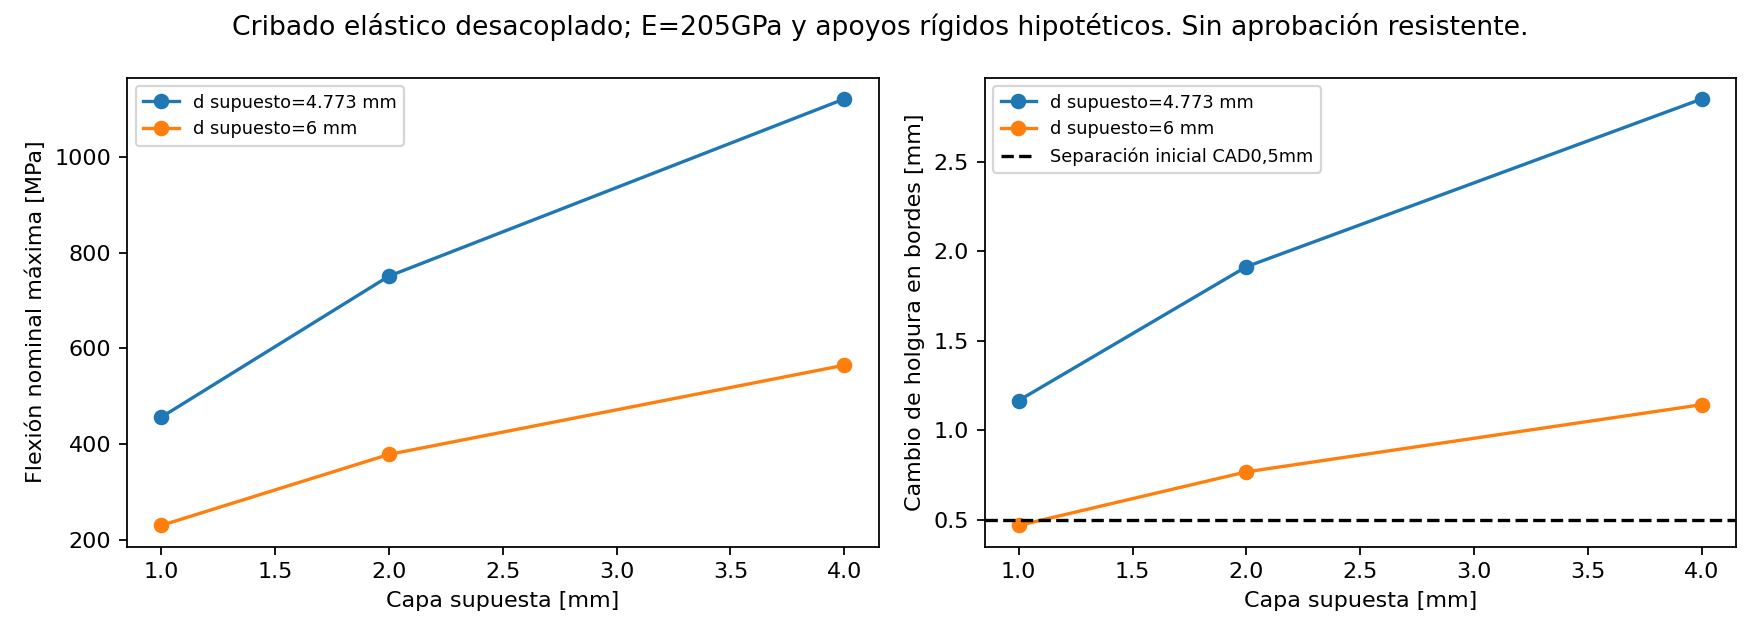
\includegraphics[width=0.95\linewidth]{eje_flecha_y_holgura.png}
\caption{Sensibilidad de flexión y variación geométrica de holgura; no son mediciones.}
\end{figure}
La traslación de los rodamientos y su diferencia se proyectan sobre el rodillo rígido,
estimando traslación y variación de holgura en bordes; se omite deformación de matriz y carcasa.
No se itera el contacto hasta definir las interfaces y propiedades.
\subsection{Rodamientos, árbol y soporte}
\begin{align}
P_{eq}&=\left(\sum_jw_jP_j^3/\sum_jw_j\right)^{1/3},&L_{10}&=(C/P_{eq})^3,\\
L_{10h}&=10^6L_{10}/(60n),&S_0&=C_0/P_{0,\max},\\
\sigma_z&=4F/(\pi d^2),&\tau_t&=16T/(\pi d^3),\\
\sigma_{\mathrm{VM},zT}&=\sqrt{\sigma_z^2+3\tau_t^2},&p_{\mathrm{proy}}&=R/(d_h t).
\end{align}
La comparación 608 supone $F_a=0$, pesos angulares uniformes y rodadura ideal al radio central,
con velocidades de matriz supuestas de $10$ y $30\,\mathrm{rpm}$. No es vida del montaje real.
La sección de árbol supone toda la carga axial y torque en el diámetro liso CAD;
la raíz real y la flexión deben resolverse antes de una comprobación resistente.
La presión proyectada en taladros y la rigidez $k\geq R/\delta$ son requisitos condicionados;
$\delta=0,05\,\mathrm{mm}$ es presupuesto ilustrativo, no tolerancia aprobada ni módulo mínimo de ABS.
No existe factor de seguridad calculable para el producto comprado sin propiedades identificadas.
Para el diseñoABS se compara $p/E_c$ únicamente como indicador uniaxial homogéneo y
$A/L\geq k/E_c$ como requisito de un apoyo ideal a compresión. Ninguno resuelve la flexión,
contacto concentrado o anisotropía de la carcasa real; no son desplazamientos predichos de la pieza.
